\section{Electronics, DAQ and Cooling}
\label{chap:TPC_sec:electronics}
Most recent update: 2020-05-12 \\
Contact person: Leif J{\"o}nsson (email: leif.jonsson@hep.lu.se)

\subsection{Introduction}
The readout electronics for the TPC has to be adapted to the design of the tracking chamber and the beam structure of the collider. The physics goals of the ILC requires high momentum resolution and two-track separation, which drive the track reconstruction in the $r\text{-}\varphi$-plane to pad sizes of small dimensions. For the $r\text{-}z$-plane a short shaping time and a high sampling rate is necessary to provide the best possible timing information. However, at the same time the noise level has to be kept at a manageable level. The sampling depth has to match the sampling frequency in order to cover the full drift length. The front end electronics has to be accommodated within pad modules, with a channel occupancy that is smaller than the pad size to allow space for the mounting frame, the voltage supply and the cooling system.

The power consumption of the front-end electronics should be kept low such that the heat dissipation does not lead to a temperature increase in the TPC-gas of more than typically \SI{1}{\degreeCelsius} after cooling. In this respect, power pulsing, where the front-end electronics is switched off for about \SI{199}{ms} between the bunch trains, helps significantly.

The readout electronics presently under development aims to demonstrate that the channel occupancy can be made compatible with the small pad size foreseen. It is based on the CERN SALTRO16-chip (shown in Figure~\ref{fig:TPC:SaltroPic}), which integrates the analogue and digital signal processing of the incoming signals within the same compact circuit. Feasibility studies of the readout concept has to be performed with existing ASICs. This prototype system is described below. A final dedicated ASIC for the ILD TPC will have a much larger channel density and higher degree of integration of functionalities and will thus occupy less space than the present prototype electronics. The size of the die is $8.7 \times \SI{6.2}{mm^2}$ and it contains 16 readout channels. The chip is programmable with respect to gain, rise time, decay time and polarity. The sampling can be clocked at frequencies 5, 10, 20 and \SI{40}{MHz} and it allows for power pulsing.

\begin{figure}
    \centering
    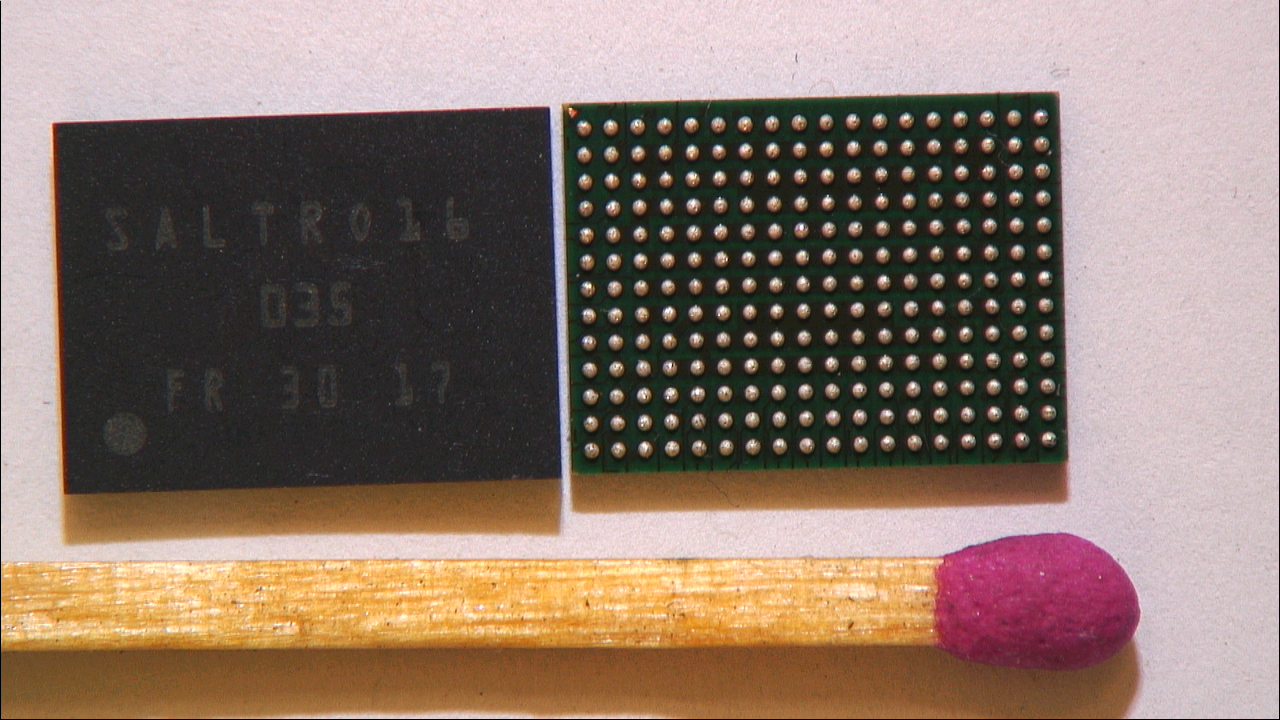
\includegraphics[width=.5\linewidth]{Tracker/TPC_Bonn/plots/TPC-Electronics_JonssonsALTRO_Chip-Photo_07062018}
    \caption{Photograph of two SALTRO-16 chip side-by-side and a matchstick for comparison.}
    \label{fig:TPC:SaltroPic}
\end{figure}

In total 840 untested dies have been obtained and delivered to the company, which performs the packaging into small capsules of size $12\times\SI{9}{mm^2}$. The bottom side of the chip contains small tin balls organized in a BGA pattern for soldering of the packaged SALTRO16 chip on so-called Multi-Chip Modules (MCM).

Eight SALTRO16 chips are mounted on an MCM, which also contains a CPLD (Complex Programmable Logic Device) controlling the data flow. The MCM-board is the smallest unit in the front end electronics and it is attached to the pad plane via four micro-connectors, whereas on the opposite side of the board there are two connectors, via which the low voltage is distributed and the signals are transmitted. The MCM-board is designed in High Density Interconnect (HDI) technology, by which the number of layers is significantly reduced compared to conventional PCB design. The dimensions of the MCM-board are $32.5 \times \SI{25}{mm^2}$ and serves 128 readout channels. This corresponds to a channel occupancy of about $\SI{6.4}{mm^{2}}$, although some space is also required for the high voltage connectors of the gas amplification system (GEMs and Micromegas) and the cooling system.

A serial readout system is used for the signal transfer to the DAQ computer. The MCM-board and the Scalable Readout Unit~\cite{1748-0221-8-03-C03015} (SRU) communicate directly via the Data Trigger Control (DTC) link. Communication, data transfer and control, between the SRU and a DAQ computer is done via Ethernet.

Cooling of the front end electronics is a challenge since the size of the cooling system must match the smallness of the electronics and still provide efficient cooling. The total power consumption of an MCM-board in continuous operation
is \SI{3203}{mW} on the top side and \SI{3028}{mW} on the bottom side. In power pulsing mode, with a bunch train of \SI{725}{\micro s}, containing 1312 bunches, the power dissipation is reduced to about \SI{223}{mW} per MCM-board on the top side and \SI{48}{mW} on the bottom side. A cooling system with cooling pipes that run on top of the MCM-boards, using two-phase \ce{CO2} coolant, is considered. Another possibility would be to use micro-channel cooling, which has been developed by the semiconductor community. Such systems are presently further developed within the AIDA2020 project, for applications in high energy physics experiments. The ILC cycle is not realistic in a test beam environment as at e.g. DESY. To get a reasonable trigger rate is e.g. a cycle with \SI{5}{ms} beam at \SI{10}{Hz} more useful, which corresponds to \SI{343}{mW} per MCM-board on the top side and \SI{168}{mW} on the bottom side, in power pulsing mode.

\subsection{Recent Milestones}
A system for testing the SALTRO-16 chips has been built and debugged. We are aiming at a readout system with at least 10,000 channels, which requires a yield of about 75\%. The tests of two pre-series have been completed. The first one, containing 34 chips, gave a lower yield, requiring an improved bonding procedure. The second pre-series, containing 55 chips, gave a yield well above the goal and we decided to go ahead with the full production.
The delivery of the bulk of the chips happened at the end of the year 2018.
The design of the final 16-layer MCM-board was completed and the boards were manufactured. By pushing the boundaries of commercially available assembly techniques to the limit, read-out of sensor pads, as small as \SI{6.3}{mm^2}, could be achieved with the MCM-board connected parallel to the pad plane. We have simplified the design by reducing the number of separate voltage levels needed from seven to two. Initial tests revealed some bugs in the PCB design, most of which could be fixed. Prior to the performance tests of the MCM-board, a prototype LV board, providing low voltage supply for a single MCM-board, was designed and produced. The design of the final LV-board intended for five MCM-boards is well under way.
For tests of the performance, two MCM-boards were mounted by the DESY electronics group at the end of 2019. The tests showed that data could be read and written and thus the concept was proven to work. Pedestal runs were performed and gave good results, and the noise performance was promising. However, this first prototype of the readout board required some corrections, which have been implemented and the next version of the MCM PCB has been ordered. The official delivery time was 8.5.2020, but at the time of writing the supplier claims a delay of about one week. The assembly by the DESY electronics group will follow together with further tests.

\subsection{Engineering Challenges}
The final aim is to produce front end electronics, high voltage supply and a cooling system which are compatible with a pad size of $1 \times \SI{6}{mm^2}$. The compactness of the electronics and the space limitations are major challenges, as well as designing a suitable and efficient cooling system. An elegant solution for the low voltage supply has to be found and due to space limitations the design of the mechanical support for the electronics is also a challenge.

\subsection{Future Plans}
In case the upcoming tests are successful, a fully mounted MCM-board will be produced and tested.
Until we have got help with the FPGA-programing we will not be able to test the rest of the chips and
thus no further MCM-boards can be produced.
The design of the micro-channel cooling support structure is ready and production is planned.
